\subsubsection{Liquid}
\noindent Liquid\cite{Liquid} is a sidechain of BTC and a typical representative of the multi-signature notary mechanism. It is designed to meet the BTC fast transfer needs of exchanges, market makers and brokers. Therefore, Liquid uses the multi-sig federation mechanism to confirm the transaction block, which can greatly improve the transaction speed.\\
\noindent Liquid based on Element codebase and uses Strong Federation technology to support 1:1 Bitcoin exchange. The basic process of the transaction is described as Figure \ref{fig:multisig}. The confirmation of this asset transfer requires multi-signature from the majority of notaries.

        \begin{figure}[H]
        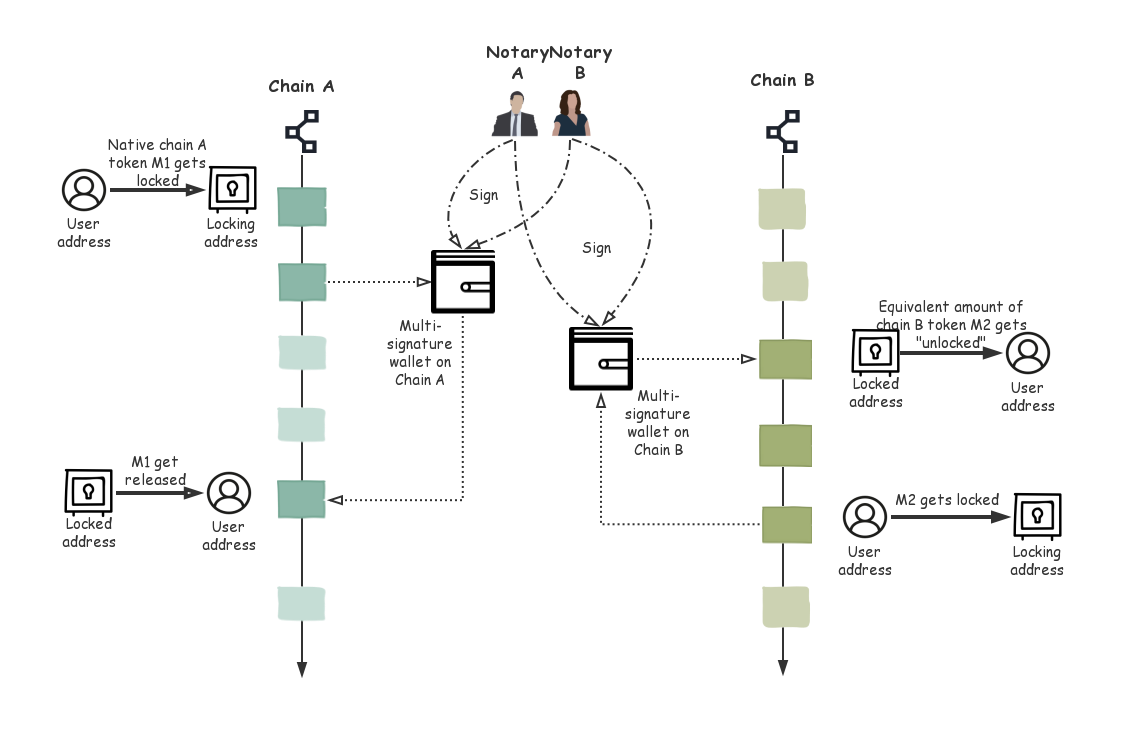
\includegraphics[width=1\textwidth]{./figures/multi_sig.png}
        \centering
        \caption{Multi-signature federation scheme}%\protect\footnotemark}
        \centering
        \label{fig:multisig}
        \end{figure}
        
\noindent In Strong Federation, there are 2 types of node role in the network:
\begin{itemize}
    \item Blocksigners: Signature verification for transactions in the sidechain to achieve block consensus. 
    \item Watchmen: When the asset is transferred from the sidechain to the main chain, it is responsible for signature verification of the transaction on the main chain, indicating that the sidechain asset has indeed been destroyed, and the main chain can unlock the corresponding number of assets.
\end{itemize}

\begin{large}
\textbf{Fusion}
\end{large}\cite{fusion}\\


\noindent Similar to the principle of Wanchain, Fusion's goal is to build a basic platform for the operation of encrypted financial applications based on blockchain technology. On this platform, a variety of tokens can be freely interacted through smart contracts to achieve value interoperability. Support multi-platform cross-chain asset transfer, using a distributed signature notary model for cross-chain transaction processing.\\

\noindent Based on Hierarchical Hybrid Consensus Mechanism(HHCM), Fusion combines the advantages of PoW and PoS consensus mechanism, which balancing the safety, efficiency, and scalability. It is the only cross-chain platform that offers parallel computing, multiple triggering mechanisms, and off-chain data support.\\

        \begin{figure}[H]
        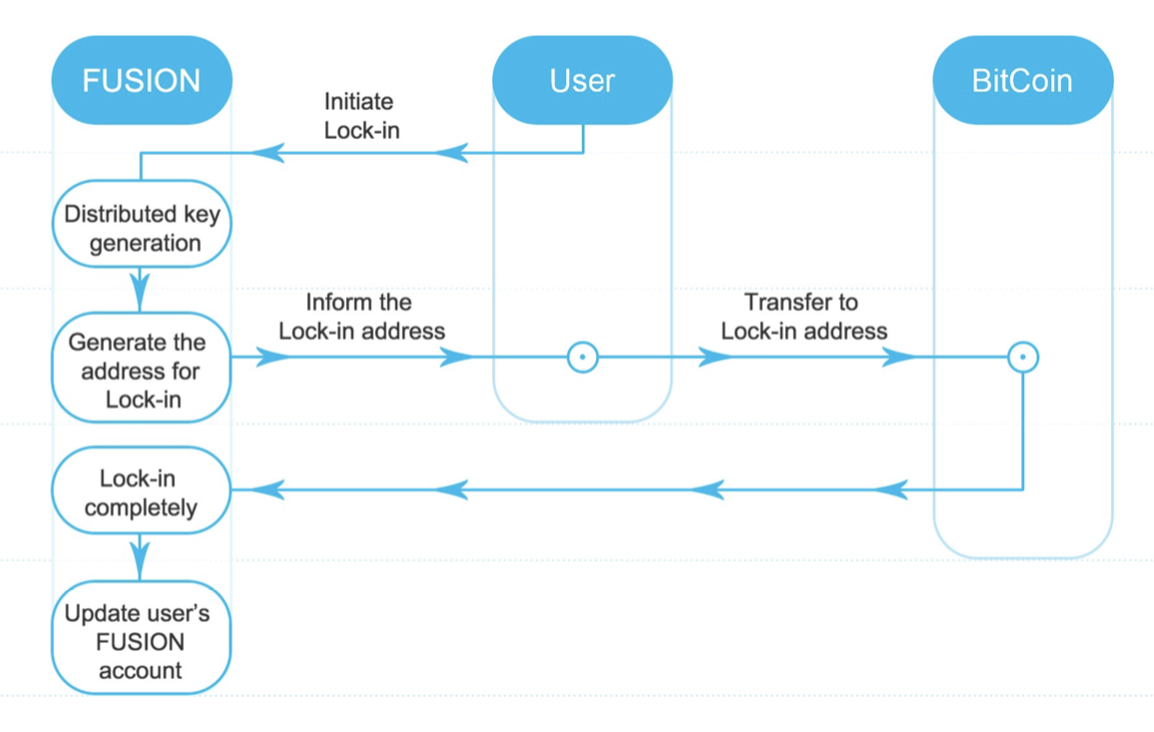
\includegraphics[width=1\textwidth]{./figures/lockin}
        \centering
        \caption{{Fusion Network Architecture, lock-in process}\protect\footnotemark}
        \centering
        \label{fig:lockin}
        
        \end{figure}
\footnotetext{Image courtesy of Fusion white paper\cite{fusion}}
\noindent The realization of cross-chain assets transaction is based on the lock-in\&lock-out process as shown in Figure \ref{fig:lockin}.



\subsubsection{ICON}
\noindent ICON\cite{icon} is committed to building a cross-chain network that connects all types of blockchain systems, enabling DApps to be interconnected across all types of blockchains. The cross-chain transactions primarily handled through notary mechanism. Figure \ref{fig:concept} below shows the overall conceptual model of ICON. With ICON, blockchains are connected around the \textbf{Nexus}, which is a loopchain-based blockchain. The whole system based on loop fault tolerant mechanism which is an enhancement of BFT-based algorithm.  \\


 \begin{figure}[H]
        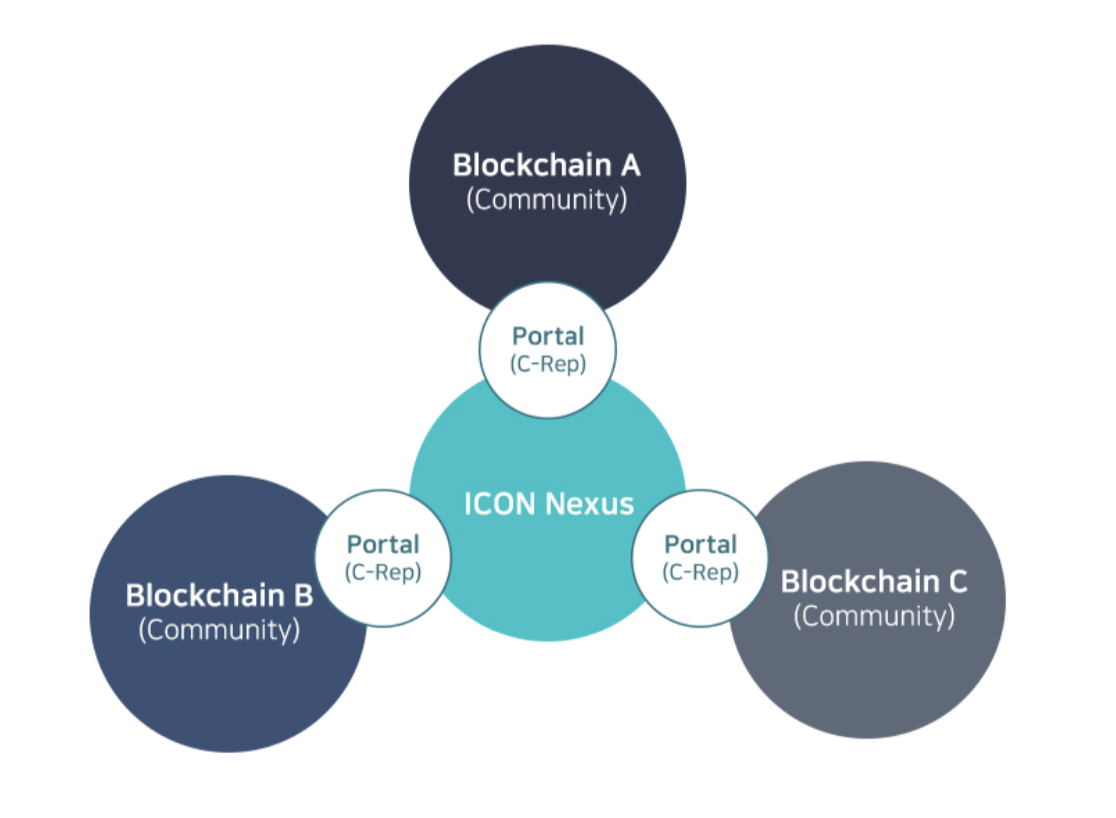
\includegraphics[width=1\textwidth]{./figures/iconconcept.png}
        \centering
        \caption{{Conceptual model of ICON}\protect\footnotemark}
        \centering
        \label{fig:concept}
        
        \end{figure}
\footnotetext{Image courtesy of ICON white paper\cite{icon}, Nexus is a Multi-Channel blockchain comprised of Light Client of respective blockchains. Each blockchain connected to Nexus via a portal.}
        \begin{figure}[H]
        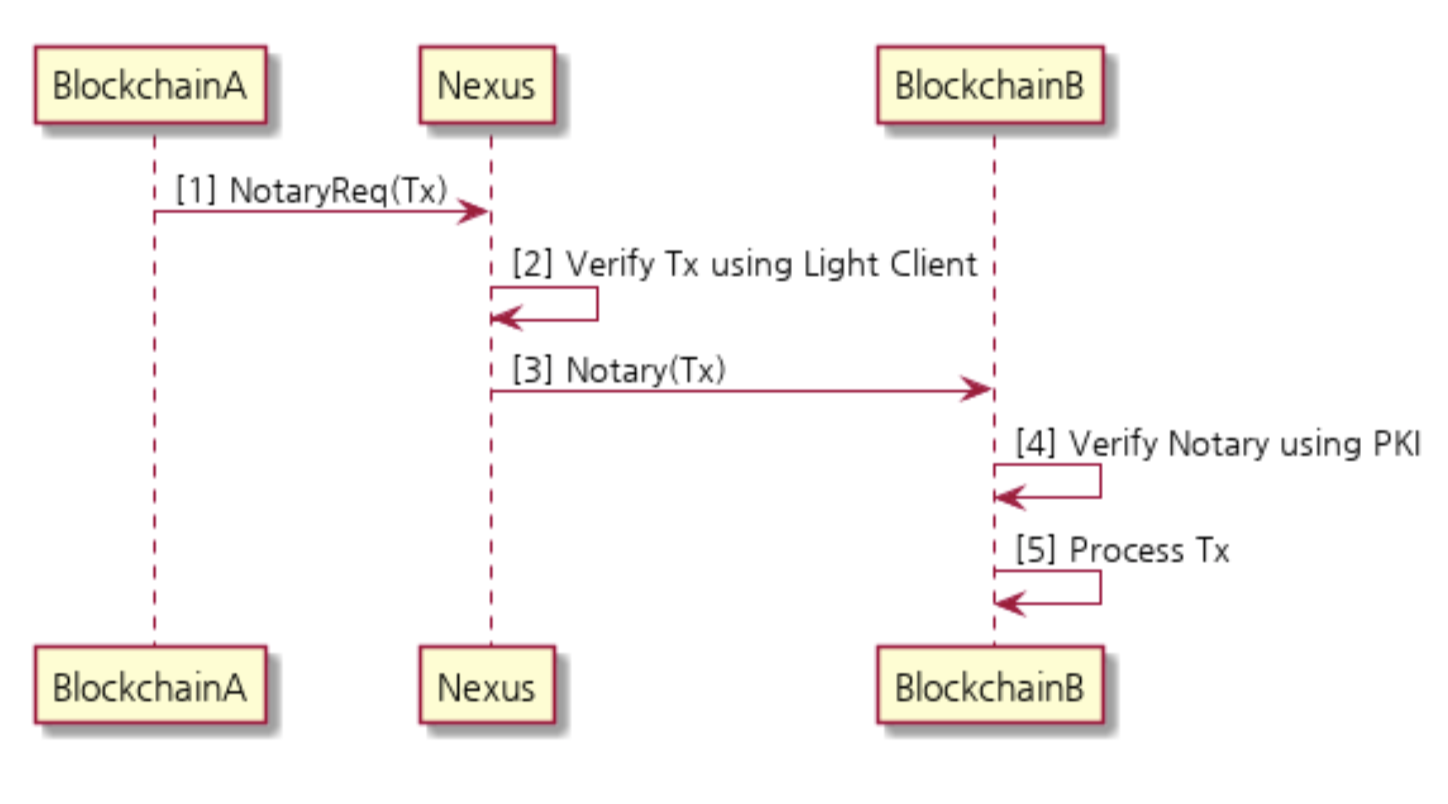
\includegraphics[width=1\textwidth]{./figures/icontrans.png}
        \centering
        \caption{{Assets transaction process through Nexus}\protect\footnotemark}
        \centering
        \label{fig:icon}
        
        \end{figure}
\footnotetext{Image courtesy of ICON white paper\cite{icon}}
\noindent Although rated as one slow progress cross-chain project, ICON still has the ambition to not only connect blockchains together but also aiming at realizing communication between the traditional ledger system and the blockchain world.


\subsubsection{AION}
\noindent Among the Interoperability Alliance\protect\footnotemark
 \footnotetext{Wanchain, ICON and AION form an alliance to overcome the technical difficulties towards cross-chain technology. reference: https://medium.com/helloiconworld/blockchain-interoperability-alliance-icon-x-aion-x-wanchain-8aeaafb3ebdd}
, AION differs from Wanchain and ICON. While the other two projects still focus on the assets and value transactions cross-chain, AION also expanding the business logic and interoperability between chains. Figure\ref{fig:aion} represents a simple multi-tier network architecture based on AION.
        \begin{figure}[H]
        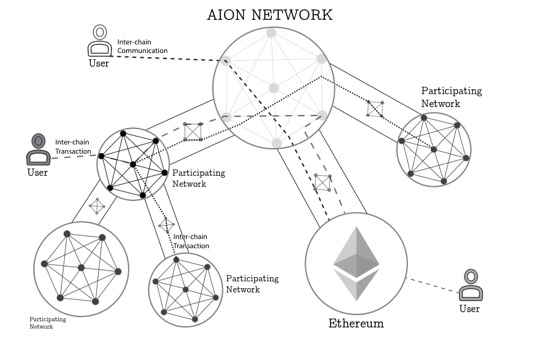
\includegraphics[width=1\textwidth]{./figures/aion.jpg}
        \centering
        \caption{{Multi-tier network structure of AION}\protect\footnotemark}
        \centering
        \label{fig:aion}
        
        \end{figure}
\footnotetext{Image courtesy of AION white paper\cite{aion}}
\noindent AION aims to establish a multi-tier cross-chain platform that supports interoperability of heterogeneous chains. By connecting networks and bridges to blockchain systems, the route of cross-chain transactions is a multi-stage process. \\
\noindent At each stage, the Validators verifies the transaction and agrees on whether the transaction is forwarded or rejected. Bridge validators will use a lightweight BFT-based algorithm to reach consensus. If a transaction is rejected at any time, any state changes due to cross-chain transactions will be revoked, at least in the connected network.\\
\noindent AION has different consensus mechanisms at different product stages, the latest AION 3.0 using mixed DPoS and PoI algorithm.\\
\noindent AION is an emerging project and still in the early stage of development.

\subsubsection{Elastos}
\noindent In order to ease the pressure on the main chain as well as provide better user experience for DApps, Elastos\cite{Elastos} adopted the main chain + sidechain architecture,  main chain only responsible for the circulation of the ELA while the DApps run on the sidechain. \\
\noindent In this scenario, the transfer of the assets between the main chain to sidechain is in a one-to-many relationship. It is feasible that the side chain only saves all the block header information of the main chain. If the main chain needs to save the block header information of all the side chains, it will lead to poor scalability. So Elastos uses asymmetric 2-way peg scheme based on SPV to realize the cross-chain function.\\
\noindent Assets from the main chain to the sidechain, Elastos using SPV proof to prove the transactions, while it secures the transfer using multi-signature notary scheme when transfer from sidechain to the main chain. We can regard this process as a combination of Plasma and Liquid.
